\documentclass[conference]{IEEEtran}

\usepackage[pdftex]{graphicx}
\usepackage{amsmath}
\usepackage{amsthm}
\usepackage{amssymb}
\usepackage{pifont}
\usepackage{graphicx}
\usepackage{caption}
\usepackage{subcaption}
\usepackage[nolist]{acronym}

\usepackage{listings}

%\usepackage{algorithmic}
\usepackage{array}

\theoremstyle{examplestyle}
\newtheorem{definition}{Definition}


\newcommand{\cmark}{\ding{51}}
\newcommand{\xmark}{\ding{55}}


\hyphenation{}

\DeclareMathOperator*{\argmin}{arg\,min}


\begin{document}




\begin{acronym}
	\acro{EM}{Expectation-Maximisation}
	\acro{ICE}{Iterative Closest Events}
	\acro{ICP}{Iterative Closest Point}
	\acro{KDE}{Kernel Density Estimator}
	\acro{RANSAC}{Random Sample Consensus}
\end{acronym}




%\title{Mining Temporal Lags in Event Sequences for Event Correlation}

\title{Mining Event Correlations and Temporal Lags in Event Sequences}


\author{
\IEEEauthorblockN{Marc-Andre Z\"oller and Marcus Baum}
\IEEEauthorblockA{Institute of Computer Science\\
University of Goettingen, Germany\\
Email: marc-andre.zoeller@stud.uni-goettingen.de,\\ marcus.baum@cs.uni-goettingen.de }
\and
\IEEEauthorblockN{
 Marco F. Huber  
}
\IEEEauthorblockA{
 USU Software AG\\ 
 R\"üppurrer Str. 1, Karlsruhe, Germany\\
Email: marco.huber@ieee.org
}
}
 



\maketitle


\begin{abstract}
Event correlation is the task to detect dependencies between events in event sequences, e.g., for predictive maintenance based on log-files.
In this work, a new data-driven, generic framework for event correlation is presented. 
First, we use a fast preliminary test statistic to determine candidate event pairs. Next, the precise distribution of the temporal lag between those pairs is determined. 
For this purpose, an new efficient iterative method is developed  that aligns two event sequences and finds the optimal  event assignments.
%Based on the assignements,  a (non-parametric) temporal lag distribution can be estimated using a Kernel Density Estimator (KDE).
In our experiments, the proposed method is much faster than state-of-the-art methods but always yields similar (or even better) results. 
\end{abstract}






\IEEEpeerreviewmaketitle



\section{Introduction}
Nearly every modern computer system provides information about its status. This status information---usually collected by logging---is often aggregated in a monitoring system for further inspection and error handling. Usually, this data can be interpreted as a sequence of events. In the most basic case an event has to have some kind of label saying what this event represents and a time stamp when the event has occurred. In addition, events are often enriched with arbitrary supplementary data such as a message, component description, or input data. A series of events can be aggregated in a sequence as illustrated in Figure \ref{fig:logToSequence}.

Events often influence and trigger each other, and hence, form a network of dependencies. With a certain complexity of the underlying system, a manual inspection and handling of all monitored events becomes quite time consuming and expensive. A major challenge during the analysis is that a single fault in an application often does not lead to a single event in monitoring. Instead, a fault---normally referred to as \textit{root cause}---often propagates through a system leading to consecutive errors depending on the first fault. This flood of events makes determination of the actual problem complicated and time consuming.

Starting from the 1980s, methods to automatically aggregate and preprocess monitored events were investigated in order to reduce the manual work. Early approaches utilize domain experts to create a knowledge database. By asking a domain expert, explicit rules and dependencies between event types are stated. Based on these rules, events are aggregated and correlated, e.g. \cite{Houck1995}, \cite{Kettschau2002}. First of all, it is not possible to transfer this system to a new domain as all rules have to be recreated. Furthermore, the creation of rules is very time consuming, difficult and error prone for non-trivial systems.

The most important generic approach utilizes time windows to find frequent event pairs, e.g. \cite{Jakobson1993}, \cite{Mannila1997} and \cite{Bouandas2007}. A time window with a fixed size is shifted over the complete sequence like an \(n\)-gram over a text. By counting how often event types occur in the same time window, frequent pairs can be found. A major drawback of this approach is that no reasonable way for choosing the window size exists. If the window size is too small, relevant event pairs may be missed. However, if the window size is too large, many false positive correlations will be detected.


The most similar approach to our work is the \textit{lagEM} algorithm proposed by Zeng et al. \cite{Zeng2015}. The \textit{lagEM} algorithm models the temporal lag between two event types \(A\) and \(B\) by a normal distribution. By using \ac{EM}, the likelihood of the model parameters---namely mean \(\mu\) and variance \(\sigma^2\)---is maximized. This algorithm is considered as current state-of-the-art and serves as a performance reference for event correlation in this work.

\begin{figure}[!tb]
	\centering
	{
	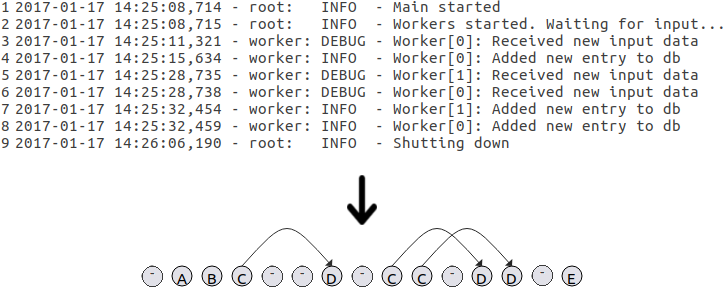
\includegraphics[width=0.45\textwidth]{images/overview.png}}
	\caption{Interpretation of a log file as an event sequence. The actual log entries are replaced by generic labels while preserving the order and time stamps of all events. Correlated events are highlighted  by arrows.}
	\label{fig:logToSequence}
\end{figure}


\textit{Event correlation} is the task to identify correlations between different event types within a sequence. By examining the dependencies between the events, a directed graph can be formed. In this graph, each node represents exactly one event type. A directed connection between two nodes means that event type \(A\) triggers \(B\). Using this knowledge it is possible to say which event types will follow after the current event predicting future states of a system. Another application is using the graph to find the root cause of a given event. Both abilities are highly desired in many domains like system monitoring, stock market, intrusion detection systems, etc. for \textit{predictive maintenance} and \textit{root cause analysis} \cite{Zeng2015}, \cite{Benferhat2008}.


\begin{figure}[!tb]
	\centering
	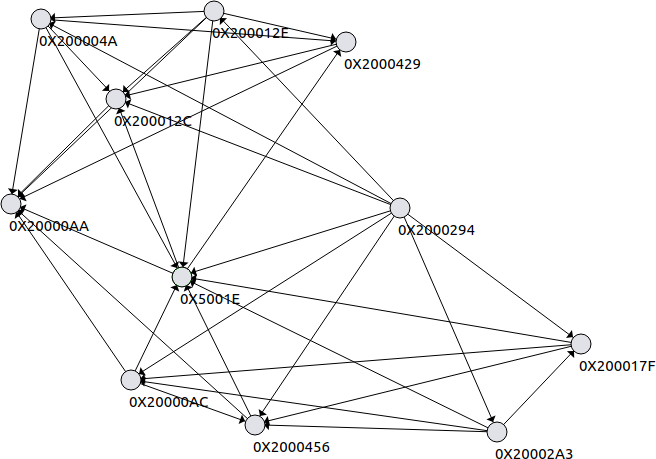
\includegraphics[width=0.45\textwidth]{images/dependency-graph}
	\caption{Example dependency graph. Each node represents an event type with a hexadecimal label. An arrow indicates a  correlation between two event types.}
	\label{fig:exampleDependencyGraph}
\end{figure}


Mathematically, the problem can be formulated as follows. Let a sequence \(\pmb{S}\) containing a set of event types \(E\) be given. Desired are all event pairs \(E_i, \; E_j \in E\) such that \(E_i\) and \(E_j\) are not independent of each other as
\begin{equation}
	P(E_i, E_j) \neq P(E_i) \cdot P(E_j)
\end{equation}
with \(P(E_i)\) the probability of \(E_i\) and \(P(E_i, E_j)\) the joint probability of \(E_i\) and \(E_j\). Those event pairs are called \textit{correlated}.

Even though independence of two events is easy to check, event correlation is difficult as neither \(P(E_i)\) nor \(P(E_i, E_j)\) are known a priori in general. This task gets even more complicated as two events do not have to appear at the same time even though they are correlated. Often, one event---called the \textit{trigger event}---happens a few seconds or minutes before the correlated event---called the \textit{response event}. For example, assume an application running on a server. The trigger event is a failure of the network card and the response event is an application alerting the lost network connection after some connection retries. The time between the network card failure and the detected network loss is called \textit{temporal lag}
\begin{equation}
	P(E_j \; | \; E_i) = \mathcal{T}_\Delta (E_j \; | \; E_i) = \mathcal{T}_\Delta (E_j - E_i)
\end{equation}
with \(\mathcal{T}_\Delta\) being an arbitrary probability density function.

In this paper, we present an event correlation method that consists of three parts:
(1) Candidate  events are identified using the energy distance. (2) A novel iterative algorithm for aligning and assigning events from two event sequences is developed. (3) A non-parametric distribution for the time lag is estimated based on a Kernel Density Estimator (KDE).
The final algorithm is in particular suitable for big data applications as it is highly efficient. 

In the next section, we will describe the proposed event correlation framework in detail.
Section \ref{sec:exp} presents an experimental evaluation of the proposed method including a comparison with the state-of-the-art.
The paper is concluded in Section \ref{sec:conc}



\section{Event Correlation Approach}
We aim at finding and analyzing correlations between pairs of different event types. In a first step, all  pairings of event types are considered and a hypothesis test is done to check if both event types are correlated or not. In order to rate the correlation between two event types,  the energy distance \cite{Rizzo2016} is used as explained in Section~\ref{sec:energyDistance}. 
If this test is positive, the actual distribution of the temporal lag is calculated. Therefore, an adapted version of the \ac{ICP} algorithm called \ac{ICE} is developed that aligns two event sequences and determines optimal event assignments, see Section \ref{sec:ice}.
Based on the result of the \ac{ICE} algorithm, a Kernel Density Estimator (KDE) determines the distribution of the time lags,  see Section~\ref{sec:labestimator}.




\subsection{Finding Candidate Events}
\label{sec:energyDistance}
The \textit{energy distance} is inspired by gravitational potential energy from physics and was recently proposed by Rizzo \cite{Rizzo2016}. Like two objects attracting each other in a gravitational field, the samples of two distributions affect each other depending on their "distance". If both sample sets were produced by equivalent distributions their potential energy is zero. To the best of our knowledge the energy distance has not yet been used for event correlation.

To compute the empirical energy distance let \(A\) be a sample set with \(m\) samples and \(B\) a sample set with size \(n\). The empirical energy distance is defined as
\begin{align}
\begin{split}
	& \text{Cor}(A, B) = \dfrac{2}{m n} \sum_{i = 1}^m \sum_{j = 1}^n \left\| a_i - b_j \right\| \\
	& - \dfrac{1}{m^2} \sum_{i = 1}^m \sum_{j = 1}^m \left\| a_i - a_j \right\| - \dfrac{1}{n^2} \sum_{i = 1}^n \sum_{j = 1}^n \left\| b_i - b_j \right\| ~.
\end{split}
\end{align}

An important property of the energy distance is that no pair-wise  mapping between \(A\) and \(B\) is required to calculate the empirical energy distance. This allows computing the correlation score without knowing event assignments. 
Consequently, only event pairs with a low energy distance can be analyzed more detailed, e.g., be determining the time lag, which lowers the computational cost significantly.

Based on the energy distance, a hypothesis test is done to check whether two events are uncorrelated (\(H_0\)).  Therefore, \(A\) and \(B\) are combined into a single sample set, randomly permuted and then split again into \(A^\pi\) and \(B^\pi\). The test statistic is defined as
\begin{equation}
	S(A, B) = T(A, A) + T(A, B) + T(B, A) + T(B, B)
\end{equation}
with
\begin{equation*}
	T(A, B) = \dfrac{m \cdot n}{m + n} \text{Cor}(A, B) ~.
\end{equation*}
Based on this test statistic, the \(p\)-value is calculated as

\begin{equation}
	p = \dfrac{1}{k} \sum_{i = 1}^k 1 \left( S(A, B) > S(A^\pi , B^\pi) \right) \enspace, 
\end{equation}
where \(k\) is the number of repetitions.



\subsection{Iterative Closest Events (ICE)}
\label{sec:ice}

We call the algorithm to match two event sequence  \acl{ICE} (\ac{ICE}) algorithm as it is an adaptation of the \acl{ICP} (\ac{ICP}) algorithm \cite{Besl1992}. \ac{ICP} is a widely-used in computer vision for point set registration, i.e., given two point clouds, \ac{ICP} searches for a rigid transformation of one point cloud to the other one. 

Given two datasets called \textit{data} and \textit{reference}, the \ac{ICP} algorithm searches for a transformation that minimizes a given cost function. This optimal transformation is calculated iteratively using the following steps \cite{Besl1992} until convergence is reached:

\begin{enumerate}
	\item \emph{Assignment Step}\\ 
	   For each point in \textit{data}, find the closest point in \textit{reference}.
	\item \emph{Transformation  Step}\\ Estimate a rigid transformation that minimizes the distance between all \textit{data-reference} pairs. Apply the estimated transformation to \textit{data}.
\end{enumerate}


In the following, we will apply the \ac{ICP} concept for matching two event sequences:

Let \(data\) be  an event sequence \(\pmb{S}_A = (a_1,\ldots, a_m)\)   of type \(A\) with \(m\) events,  and \(reference\) be an event sequence \(\pmb{S}_B=(b_1,\ldots, b_n)\)  of \(  n\) events of type \(B\) with. 
We aim at finding the temporal translation between these two event sequences as it represents the ``mean'' time lag.
Hence, the objective is to find a translation $t \in \mathbb{R}$ that minimizes 
\begin{equation}
 \dfrac{1}{m} \sum_{i = 1}^{m} \left( a_i + t - b_{\alpha_i(t)} \right)^2 \enspace , \\
\end{equation}
where $\alpha_i(t)= \argmin_j \; (a_i+t-b_j)^2$ is the index of the closest event of type  $B$  to the event $a_i$.

The \ac{ICE} algorithm starts with an initial guess $t^{(0)}$ for the translation and iteratively improves the current guess $t^{(l)}$  in two steps as described in the following.

\begin{enumerate}
 \item \emph{Assignment Step}\\
For each point in \(\pmb{S}_A\) the corresponding point in \(\pmb{S}_B\) with minimal squared Euclidean distance has to be found under incorporation of the current translation $t^{(0)}$, i.e., 
\begin{equation}
\alpha_i(t^{(l)})= \argmin_j \;  (a_i+t^{(l)}-b_j)^2  \enspace .
\end{equation}
This calculation is normally done by computing all pairwise distances and selecting the smallest one. It is important to note that several points in \(\pmb{S}_A\) can be assigned to the same point in \(\pmb{S}_B\) and that some points in \(\pmb{S}_B\) can remain unpaired.  



\item  \emph{Translation  Step}\\
With the pairwise correlations given, the optimal translation can be calculated by solving  the optimization problem
\begin{equation}
t^{(l+1)}= \argmin_{t} \;  \dfrac{1}{m} \sum_{i = 1}^{m} \left( a_i + t - b_{\alpha_i(t^{(l)})} \right)^2 \enspace , \\
\end{equation}
using the  least squares formulas.
 
\end{enumerate}




Naively implemented, these two steps run in \(\mathcal{O}(m \cdot n)\) as all pair-wise distances have to be calculated. However, several techniques exist to improve the \textit{data-reference} assignment using \(k-d\) trees or caching \cite{Pomerleau2015}. Furthermore, it can be proven that the number of iterations is also limited by \(\mathcal{O}(m \cdot n)\) as the input samples are one-dimensional \cite{Ezra2008}.

\ac{ICE} calculates one translation for all \textit{data} points. As a consequence, outliers can influence the optimization process. To counter the effects of additional points in \(\pmb{S}_A\), a random sampling of \textit{data} is done before calculating the best pairs. If the rough number of outliers is known in advance, \textit{data} can be simply trimmed by their distances \cite{Chetverikov2002}. However, if the amount of outliers is not known---as it is usually the case---this approach is not reasonable. For this situation it is better to adjust the used samples dynamically. A quite simple approach is performing plain outlier removal using \(z\)-scores and thresholding \cite{Phillips2007}. Unfortunately, additional points in \(\pmb{S_B}\) cannot be easily sorted out.


As an iterative algorithm, \ac{ICE} finds a local minimum \cite{Do2008}. Consequently, it is important that optimization starts close to the true solution to ensure a global minimum. In order to obtain a good initial guess, a \ac{RANSAC} \cite{Fischler1981} algorithm is used:
\begin{enumerate}
	\item Select \(n\) sample points randomly from \(\pmb{S}_A\). Ensure that all sample points have a minimal distance \(d\) to limit the effects of local distortions.
	\item For each selected sample point find the \(k\) nearest neighbors in \(\pmb{S}_B\) and select one of these at random.
	\item Based on these \(n\) pairs, compute the rigid transformation as usually in \ac{ICE}.
\end{enumerate}

These three steps are repeated \(q\) times and the translation with the minimal error is used as initial guess. This method ensures that, with very high probability, the initial guess is not influenced by outliers. If a priori information about the true distribution is given, this knowledge can be used to enhance the initial guess. This allows basic incorporation of additional knowledge.


\subsection{Time Lag Estimator} \label{sec:labestimator}
Based on the final assignments $\alpha_i(t^*)$ and the final transformation $t^*$, the time lag distribution is calculated. Each event pair is interpreted as a sample. The samples are used to train a \ac{KDE} with
% \begin{equation}
% 	\label{eq:solutionICP}
% 	P(B \; | \; A) = \hat{f}_h \left(
% 		\left[
% 			b_{\alpha_i(t^*)} - a_1 + t \;
% 			\dots \;
% 			b_{\alpha_i(t^*)} - a_m + t
% 		\right] \right)~.
% \end{equation}
\begin{equation}
	\label{eq:solutionICP}
 f_{\text{Lag}}(t) = \tfrac{1}{m}  \sum_{i=1}^m  K\left( \frac{t+ b_{\alpha_i(t^*)} - a_i }{ h} \right)  \enspace ,
	\end{equation}
with Gaussian kernel function $K(\cdot)$ and bandwidth $h$ that is selected by Scott's rule-of-thumb~\cite{Scott1992}.











\section{Experiments} \label{sec:exp}
%TODO distances neu berechnen

This section is devoted to a performance evaluation based on synthetic and real data. The correlated event types are identified using the energy distance as described in Section \ref{sec:energyDistance}. Furthermore, all detected correlations are evaluated against the  ground truth both visually and based on the energy distance.
We compare the time lags obtained from the  \ac{ICE} approach  with \textit{lagEM} \cite{Zeng2015}. %For using the \textit{lagEM} algorithm, an initial guess of \(\mu\) and \(\sigma\) has to be given. 
Zeng et al. suggest to  initialize \(\mu\) and \(\sigma\) for  \textit{lagEM} randomly \cite{Zeng2015}. Hence, for all  experiments, the initial mean is generated from a uniform distribution \(\mathcal{U}(0, 100)\) and all correct means are also in \([0, 100]\).





\subsection{Synthetic Sequences}
At first,  two synthetic sequences  are generated and analyzed as described in the following.
\paragraph{Scenario 1}
For the first synthetic sequence, an experiment used by Zeng at al.  \cite{Zeng2015} is considered (see  Table I): A sequence contains $200$ elements in total. Event \(A\) occurs based on an exponential distribution with \(\beta = 27.5\). Event \(B\) follows after event \(A\) with a normally distributed time lag \(\mathcal{N}(77.01, 6.664)\). All events are lost with a probability of 10\%.


\begin{figure}[!tb]
	\centering
	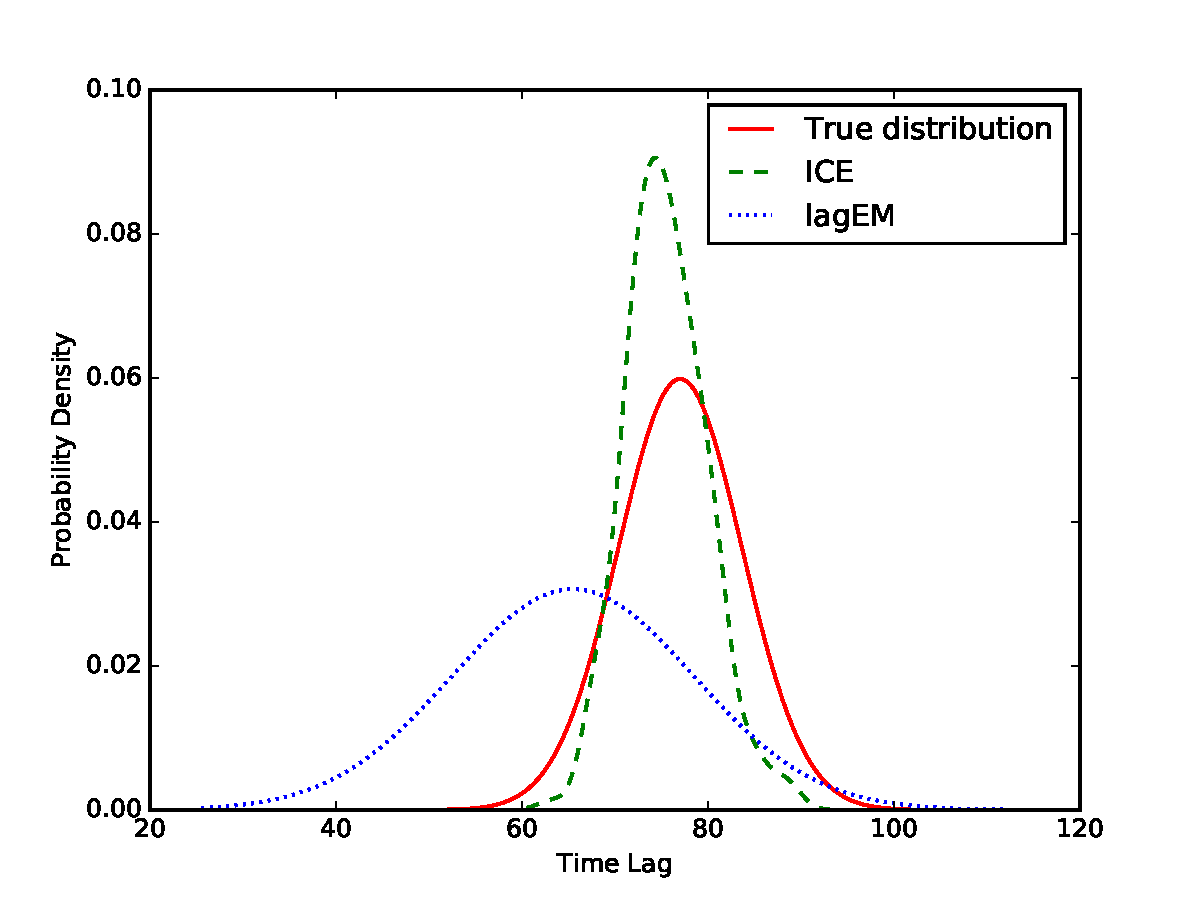
\includegraphics[scale=0.4]{images/scenarios/1.pdf}
	\caption{Estimated distributions for scenario 1.}
	\label{fig:scen1}
\end{figure}

Figure \ref{fig:scen1} shows the estimated distributions for both matchers. Even though nearly all event pairs overlap, \ac{ICE} ($0.0509$) is able to estimate the true distribution. Even with several retries, \textit{lagEM} was not able to estimate the correct distribution, which is also reflected in the calculated distance of $0.3209$. Zeng et al. reported the same behavior but were able to solve it by using longer sequences \cite{Zeng2015}.



\paragraph{Scenario 2}
This scenario introduces two additional event types. Furthermore, the temporal lag is not modeled by normal distributions: A sequence contains $1000$ elements in total. Event \(A\) occurs based on an uniform distribution with \(\mathcal{U}(30, 50)\). Event \(B\) follows after event \(A\) with an exponentially distributed time lag with \(\beta = 10\) and an offset of $25$. Independently of \(A\) and \(B\) an additional event pair exists. Event \(C\) occurs based on an exponential distribution with \(\beta = 25\) and an offset of $10$. Event \(D\) follows after event \(C\) with a uniformly distributed time lag \(\mathcal{U}(15, 25)\). Again, all event types are lost with a probability of 10\%.


\begin{figure}[!tb]
	\centering
	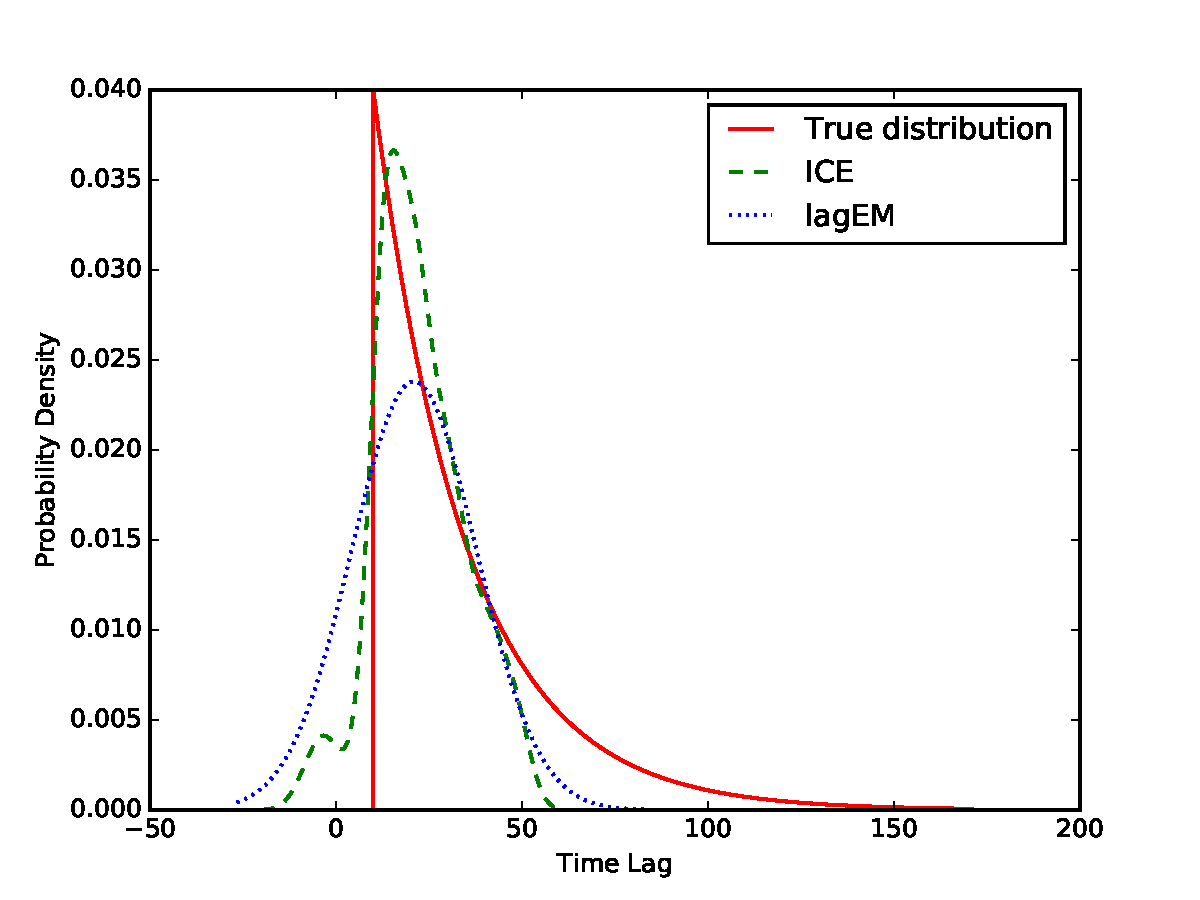
\includegraphics[scale=0.4]{images/scenarios/2-AB.pdf}
	\caption{Temporal lag between event \(A\) and \(B\) in scenario 2.}
	\label{fig:scen2-1}	
\end{figure}

\begin{figure}[!tb]
	\centering
	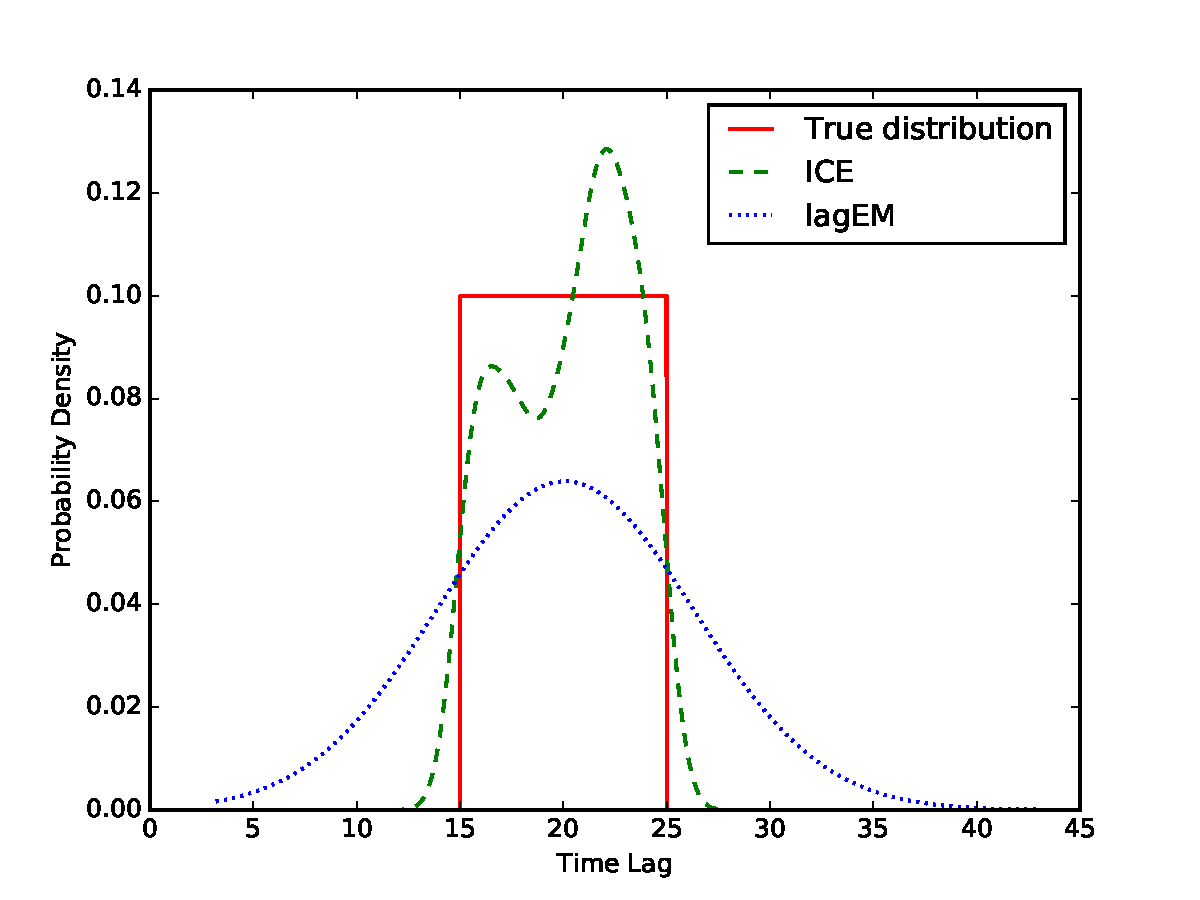
\includegraphics[scale=0.4]{images/scenarios/2-CD.pdf}
	\caption{Temporal lag between event \(C\) and \(D\) in scenario 2.}
	\label{fig:scen2-2}	
\end{figure}

First of all, the hypothesis test using the energy distance is able to detect only correlations between the event types \(A \leftrightarrow B\) and \(C \leftrightarrow D\). Figure \ref{fig:scen2-1} shows the estimated distributions between event \(A\) and \(B\). Basically, both algorithms are able to estimate the correct distribution quite well. \ac{ICE} misses the trailing event pairs. Consequently, the distance is quite large with $0.0675$. The \textit{lagEM} algorithm estimates the mean precisely. But the probability of small or even negative time lags is overestimated. This is caused by the inherent assumption that the temporal lag is normally distributed. Nevertheless, the estimate is still slightly worse than \ac{ICE} with $0.0938$.

The same behavior can be observed in Figure \ref{fig:scen2-2} for the temporal lag between \(C\) and \(D\). \textit{lagEM} estimates the correct mean. However, the variance is too big as it is hard to approximate a uniform distribution with a normal distribution. This yields a higher distance of $0.0547$. In contrast, \ac{ICE} ($0.0052$) is able to estimate the correct distribution better. The jittery probability density can be explained by the limited number of samples.












\subsection{Symantec Log}
\label{sec:symantecLog}

After using synthetic data for testing the performance, the next step is to use real world data. Therefore, an event log of \textit{Symantec Endpoint Protection Client} was collected and analyzed. The event log contains events from 5. March 2015 to 10. March 2016. In total, the log contained 3742 events of 19 different types.



First, it was tested which correlations are detected by a hypothesis test using energy distances with a significance level \(\alpha = 0.05\). In the following some exemplary detected correlations are listed. The true distribution and the estimates by \ac{ICE} and \textit{lagEM} are displayed. The time lag in seconds is divided by 100 for better readability.


\paragraph{\textit{7} \(\leftrightarrow\) \textit{66}} It is reasonable to assume that the download of a new virus definition triggers an antivirus scan. Yet, event 7 occurs roughly ten times more than event 66. During a manual inspection multiple correlation were detected.

\begin{figure}[!tb]
	\centering
	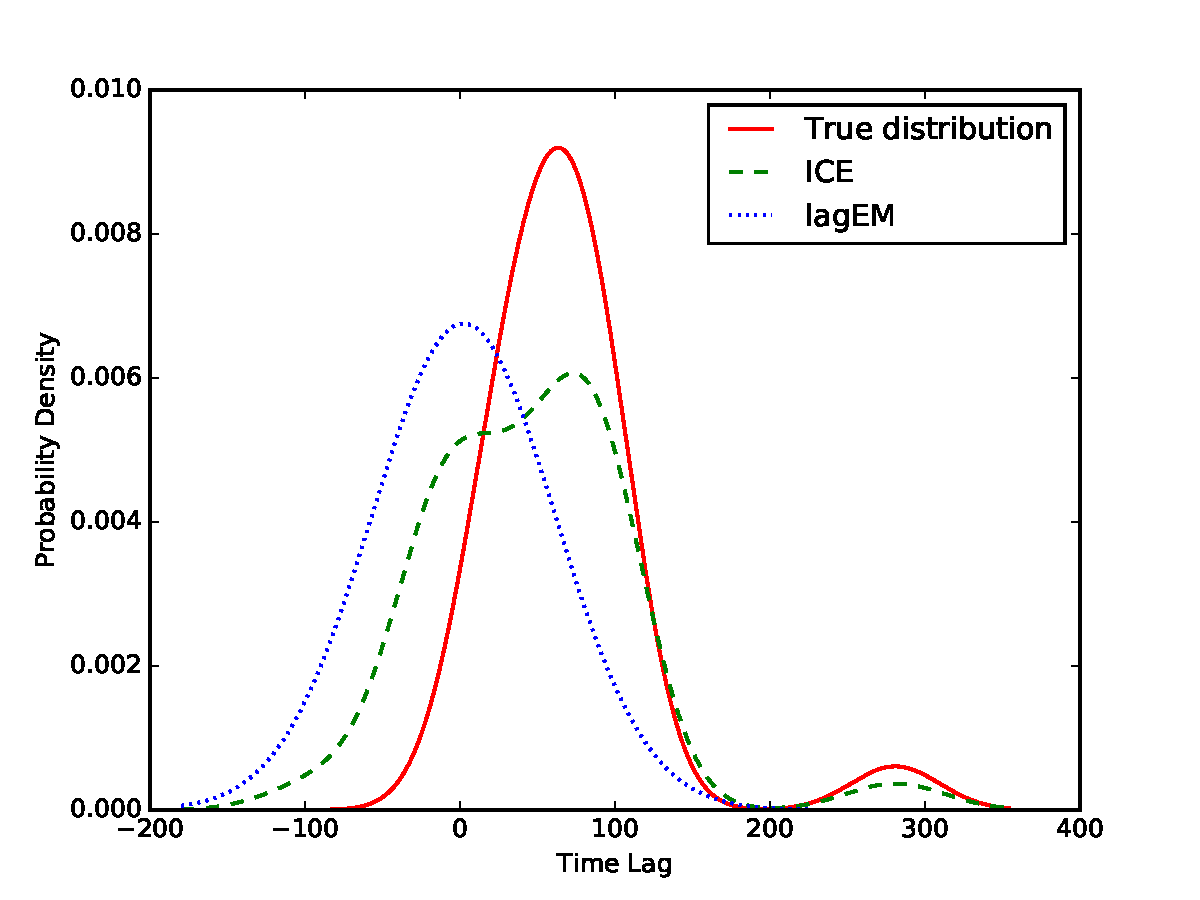
\includegraphics[scale=0.4]{images/symantec/7-66.pdf}
	\caption{Distribution of the temporal lag between event 7 and~66.}
	\label{fig:7-66}
\end{figure}

Figure \ref{fig:7-66} shows the detected correlations of \ac{ICE} and \textit{lagEM}. All algorithms estimate the main peak of the true distribution quite good. However, no algorithm is able to estimate the true distribution completely correct. The \textit{lagEM} algorithm underestimates the mean, \ac{ICE} estimates a second peak around zero. These observations are also visible via the energy distance: \ac{ICE} calculates a better result (0.0805) than \textit{lagEM} (0.3854).




\paragraph{\textit{65} \(\leftrightarrow\) \textit{66}} A correlation between the start and stop of an antivirus scan is quite obvious. A manual inspection of the log file revealed a connection between several event types. At some point an antivirus scan is started (event 3). This scan runs for roughly one hour until it is suspended (event 65). On the next Friday the virus scan is resumed (event 66) for one hour and suspended again. This is repeated until the scan eventually completes (event 2) and a new scan is started one week later. During the inspection 27 correlated event pairs were identified. The remaining 20 events are not correlated leading to roughly \textasciitilde 38\% outliers. Nevertheless, \ac{ICE} is able to exactly detect the correct correlations.

\begin{figure}[!tb]
	\centering
	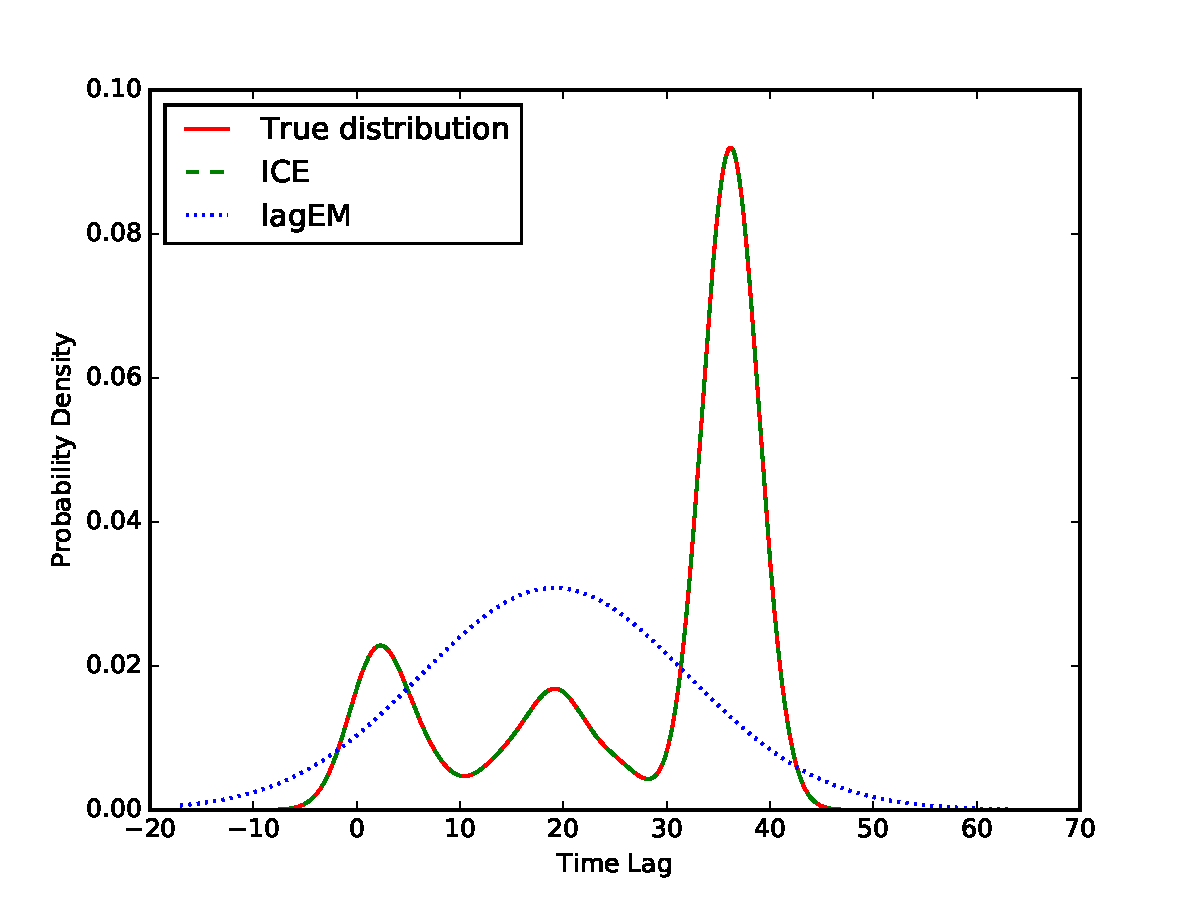
\includegraphics[scale=0.4]{images/symantec/66-65.pdf}
	\caption{Distribution of the temporal lag between event 65 and~66.}
	\label{fig:66-65}
\end{figure}

Figure \ref{fig:66-65} also shows the estimated time lag by the \textit{lagEM} algorithm. This algorithm computes a time lag distributed by \(\mathcal{N}(19.125, 12.9365)\) leading to a distance of $0.1314$. However, it is important to note, that the \textit{lagEM} algorithm was initialized with a \(\mu\) close to the correct solution. Even though the rough distribution is estimated quite well, the estimate of \ac{ICE} resembles the true distribution perfectly - yielding a distance of $0$. This is a very impressive  as the data set contains roughly 38\% outliers.



\paragraph{\textit{2} \(\leftrightarrow\) \textit{3}} During the manual analysis of events 65 and 66, a correlation between events 2 and 3 was detected. Also the energy distance is able to detect this correlation. For this experiment \textit{lagEM} was initialized with \(\mathcal{U}(5900, 6200)\).

\begin{figure}[!tb]
	\centering
	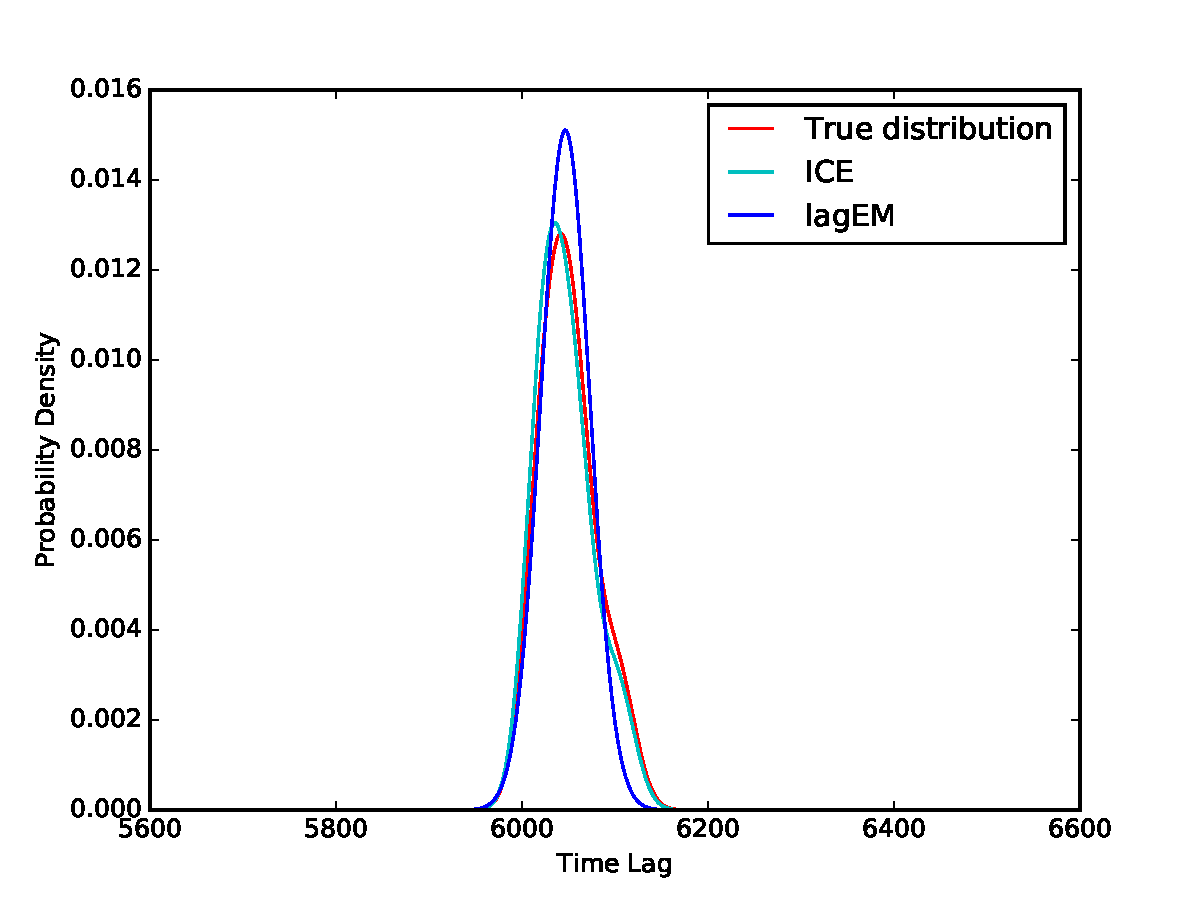
\includegraphics[scale=0.4]{images/symantec/2-3.pdf}
	\caption{Distribution of the temporal lag between event 2 and~3.}
	\label{fig:2-3}
\end{figure}

As Figure \ref{fig:2-3} shows, all algorithms are capable of detecting the rough distribution of the true time lag with a quite low distance (\ac{ICE} 0.0085, \textit{lagEM} 0.0894).


\begin{table}[!ht]
	\centering
	\begin{tabular}{c p{0.3\textwidth} c}
		\textbf{Event ID} & \multicolumn{1}{c}{\textbf{Description}} & \textbf{Count} \\
		\hline
		\textit{2}	& Symantec finishes an antivirus scan of the hard drive for malware. & 8 \\
		\textit{3}	& Symantec starts an antivirus scan of the hard drive for malware. & 10 \\
		\textit{7}	& A virus definition with new threat descriptions has been found. & 308 \\
		\textit{65}	& Symantec antivirus scan suspended. & 36 \\
		\textit{66}	& Symantec antivirus scan continued. & 38 \\
	\end{tabular}
	\caption{Excerpt of all event types in the Symantec log file with a short description and the number of occurrences.}
	\label{tbl:symantecEvents}
\end{table}


\subsection{Resource Consumption}
Besides the quality of the estimation, the resource consumption---namely runtime and memory usage---is an important evaluation factor. 


\begin{table}[!tb]
	\centering
	\begin{tabular}{c c c c}
		\textbf{Scenario} & \textbf{Algorithm} & \textbf{Runtime} & \textbf{Memory} \\
		\hline
		1	& \ac{ICE}				&	~~00:02.981	&	~~93.516927	\\
			& \textit{lagEM}		&	~~26:45.805	&	115.217656	\\
		\\
		2	& \ac{ICE}				&	~~00:12.749	&	~~94.756510	\\
			& \textit{lagEM}		&	258:32.001	&	~~95.985677	\\
		\\
		2--3 & \ac{ICE}				&	~~00:01.815	&	169.492188 \\
			&	\textit{lagEM}		&	~~00:00.297	&	169.085938 \\
		\\
		66--65 & \ac{ICE}			&	~~00:00.711	&	178.468750 \\
			&	\textit{lagEM}		&	~~00:01.342	&	178.078125 \\
		\\
		7--66 & \ac{ICE}			&	~~00:04.394	&	176.121094 \\
			&	\textit{lagEM}		&	~~00:18.022	&	176.394531 \\
	\end{tabular}
	\caption{Resource consumption of both algorithms for all scenarios. The last two columns contain the runtime in minutes and memory usage in megabytes.}
	\label{tbl:resources}
\end{table}



As Table \ref{tbl:resources} shows, \textit{lagEM} has a longer runtime than \ac{ICE}. This is effect is especially visible for many events. Concerning memory consumption, both algorithms are very similar and constant for all scenarios.



\section{Conclusion} \label{sec:conc}
We developed a new data-driven approach for event correlation that only utilizes an event time stamp and label. This framework is able to automatically detect correlated event pairs and determine the temporal lag distribution between those. It uses a  test for goodness of correlation to determine candidate event pairs before applying a time consuming matching. These candidate pairs can be processed by our new \ac{ICE} algorithm or an already existing approach like \textit{lagEM}. By examining only pair-wise event types, this framework is highly applicable to big data as all event pairs can be processed in parallel.

For calculating the temporal lag distribution between two event types, a new algorithm \ac{ICE} has been proposed. This approach does not require any  prior information, e.g. a good initialization or domain knowledge. Furthermore, no inherent assumptions about the true distribution of the temporal lag is included making it highly flexible. While often obtaining results better than state-of-the-art approaches, the runtime is also significantly less. Instead of a few hours calculation time, results are available within seconds.

Tests with simulated data and a real data set demonstrated the performance of the presented method. Using the Symantec log, several diverse and highly complex temporal lag distributions have been estimated and analyzed. This data set demonstrated the advantage of eliminating assumptions about the true distribution from the event correlation process as \ac{ICE} has  more precise results than \textit{lagEM}.

Furthermore, the data set has shown that the presented methods work with very limited sample sets--using only eight samples to estimate a distribution. However, for large sample sets--as in the simulated sequences--a fast runtime with memory consumption equal to \textit{lagEM} is obtained.



% conference papers do not normally have an appendix


% use section* for acknowledgment
% \section*{Acknowledgment}
% 
% 
% The authors would like to thank...








\bibliographystyle{IEEEtranS}
\bibliography{references}



\end{document}


